\documentclass[10pt,a4paper,titlepage]{jreport} % ドキュメントクラスを1つに統一


\usepackage[top=25truemm,bottom=25truemm,left=20truemm,right=20truemm]{geometry} % 余白設定
\usepackage[dvipdfmx]{graphicx} % 画像の挿入
\usepackage{graphicx}
\usepackage{listings} % コードリスト用
\usepackage{jlisting} % 日本語対応のリスト用
\usepackage{jverb} % 日本語のベタ打ち
\usepackage{booktabs}
\usepackage{pgfplots} % グラフ描画用パッケージ
\pgfplotsset{compat=1.18} % バージョン指定
\usepackage{float}
\parindent = 0pt % 段落の字下げを無効化

\usepackage{titlesec}
\usepackage{etoolbox}
\makeatletter
\patchcmd{\chapter}{\if@openleft\cleardoublepage\else\if@openright\cleardoublepage\else\clearpage\fi\fi}{}{}{}
\makeatother
\lstset{breaklines=true, postbreak=\mbox{$\hookrightarrow$}\space, keepspaces=true, escapeinside={\%*}{*)}}

\titleformat{\chapter}[hang] % 章のフォーマットを変更
  {\normalfont\huge\bfseries} % フォント設定
  {\thechapter} % 番号部分の表示形式
  {1em} % 番号とタイトルの間のスペース
  {} % タイトルの前に入れる内容（ここでは空）
\usepackage{xcolor}
\usepackage{amsmath}
\usepackage{amssymb} % ←これで \mathbb{R} が使える

\lstset{
  language=Matlab,              % 言語はMATLAB
  basicstyle=\ttfamily\small,   % フォントは等幅、サイズ小さめ
  keywordstyle=\color{blue},    % キーワード（function, endとか）を青
  commentstyle=\color{green!50!black}, % コメントを深緑
  stringstyle=\color{red!70!black},    % 文字列（'...'）を赤系
  numbers=left,                 % 行番号を左に表示
  numberstyle=\tiny\color{gray},% 行番号をグレーで小さく
  stepnumber=1,                 % 毎行行番号つける
  numbersep=10pt,               % コードとの間隔
  backgroundcolor=\color{gray!10}, % 背景うっすらグレー
  frame=single,                 % 枠をつける
  rulecolor=\color{black},      % 枠線は黒
  breaklines=true,              % 長い行を折り返す
  breakatwhitespace=false,      % スペースでだけ折り返すか（falseにして自然な折り返し）
  showspaces=false,             % スペースは特別に表示しない
  showstringspaces=false,       % 文字列中のスペースも普通に表示
  tabsize=2                     % タブ幅2
}


\title{C102「AI・機械学習：ニューラルネットワークによる教師あり学習」} % タイトル
\author{
  学生番号：242C2016  氏名：奥村直 \\
  \\
  知的システム工学科システム制御コース
  } % 著者
\date{\today} % 日付

\begin{document}

\maketitle

\chapter{目的}

　本演習の目的は、実際にMatlabのプログラミングを行うことにより、AI・機械学習の基
礎の一つである「ニューラルネットワークによる教師あり学習」を理解することである。

\chapter{第１週：最急降下法}

\section{演習課題1.1}

\subsection{演習課題（a）}

（a）初期値wやステップ幅epを様々な値に変更し、最急降下法での収束
がどのように変わるか確かめよ。初期値は描画範囲（-5～5の範囲）で2
刻みくらいで変更する。ステップ幅epは0.8, 0.5, 0.2, 0.1, 0.05, 
0.01 などに変更する。必要に応じて、反復回数itersも変更する。\\

\begin{figure}[H]
  \centering
  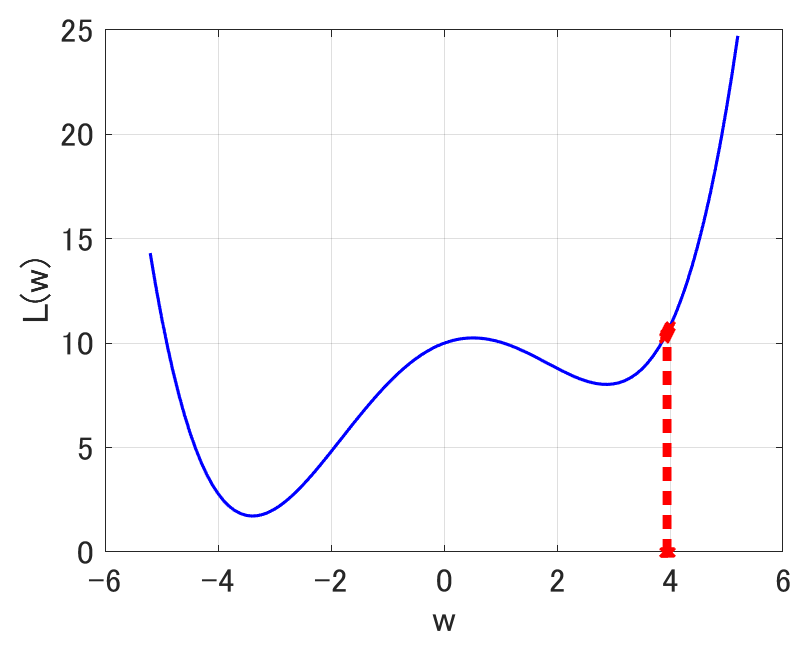
\includegraphics[width=0.8\linewidth]{w4ep0.001iters20.eps}
  \caption{w=4,ep=0.001,iters=20のときのグラフ}
  \label{fig:sample1}
\end{figure}

\begin{figure}[H]
  \centering
  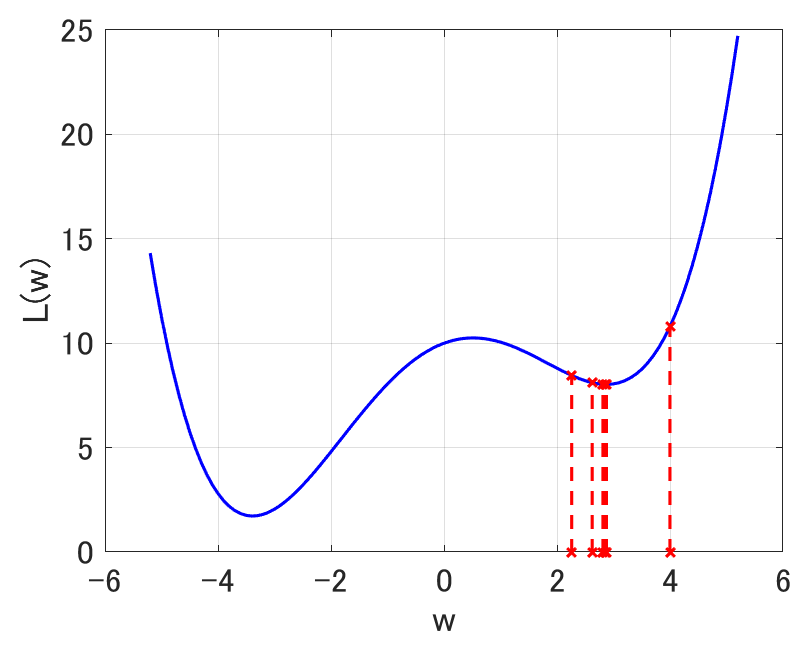
\includegraphics[width=0.8\linewidth]{w4ep0.3iters20.eps}
  \caption{w=4,ep=0.3,iters=20のときのグラフ}
  \label{fig:sample2}
\end{figure}

\begin{figure}[H]
  \centering
  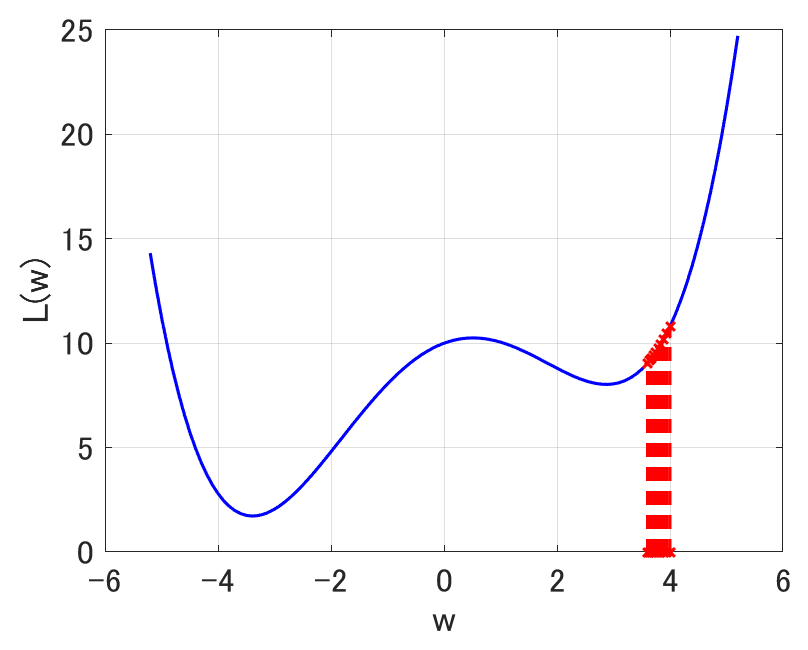
\includegraphics[width=0.8\linewidth]{w4ep0.01iters10.eps}
  \caption{w=4,ep=0.01,iters=10のときのグラフ}
  \label{fig:sample3}
\end{figure}

\begin{figure}[H]
  \centering
  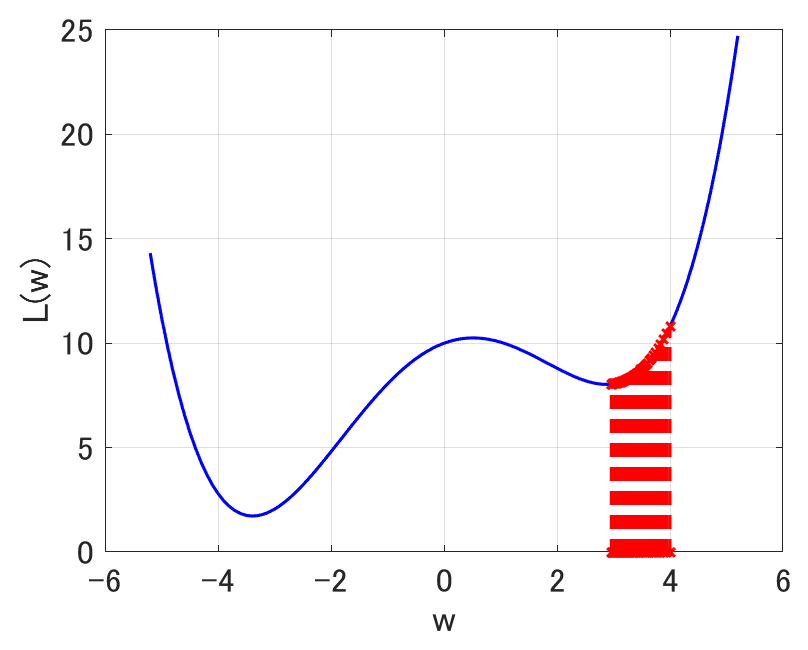
\includegraphics[width=0.8\linewidth]{w4ep0.01iters70.eps}
  \caption{w=4,ep=0.01,iters=70のときのグラフ}
  \label{fig:sample4}
\end{figure}

\begin{figure}[H]
  \centering
  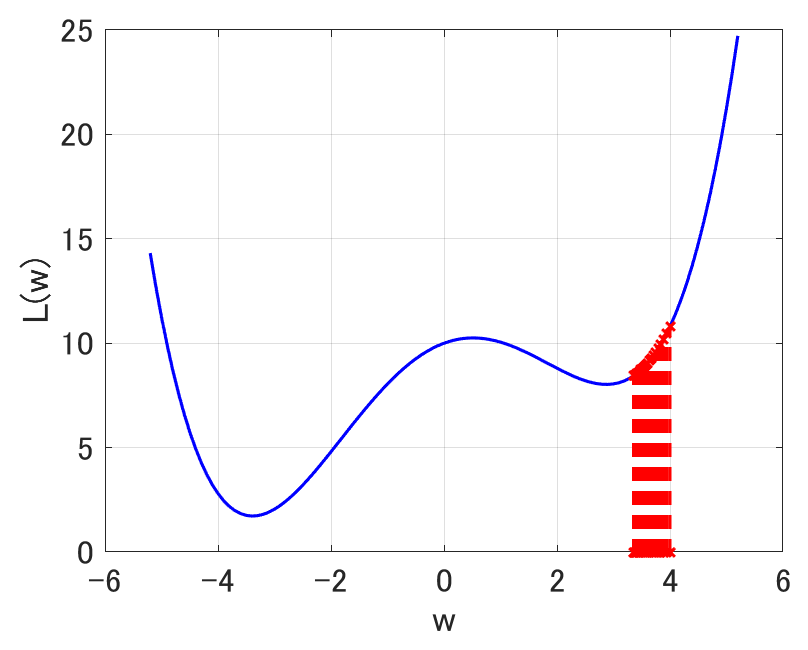
\includegraphics[width=0.8\linewidth]{w4ep0.01iters20.eps}
  \caption{w=4,ep=0.01,iters=20のときのグラフ}
  \label{fig:sample5}
\end{figure}

\begin{figure}[H]
  \centering
  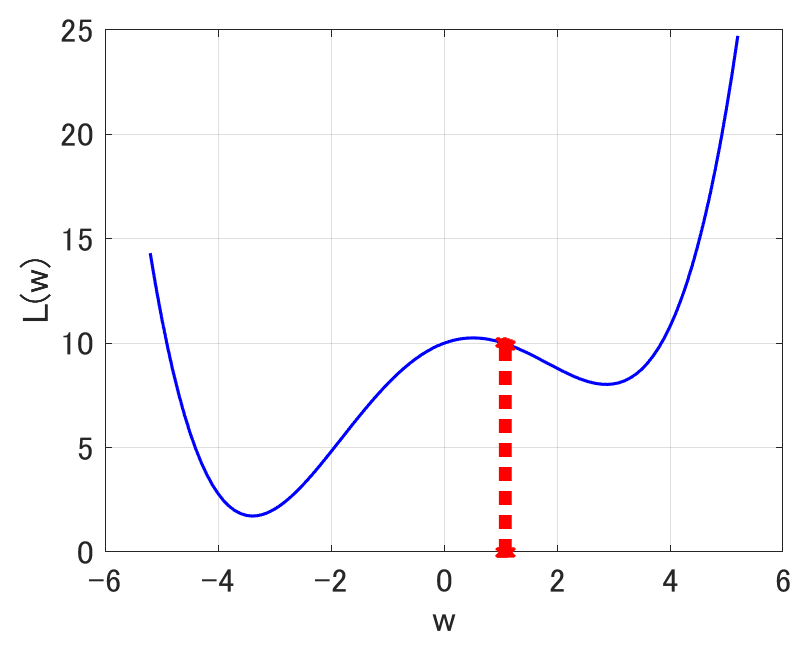
\includegraphics[width=0.8\linewidth]{w1ep0.01iters20.eps}
  \caption{w=1,ep=0.01,iters=20のときのグラフ}
  \label{fig:sample6}
\end{figure}

\subsection{演習課題1.1（b）}

（b）目的関数が

\begin{equation}
L(w) = \sin (2w) + \frac{w^2}{8} + 2
\end{equation}

の場合について、プログラムを変更して「saikyu12.m」とし、(a)と同じように
様々な初期値とステップ幅に対してどのような振る舞いになるかを確かめよ。
この場合の勾配 $\frac{ \partial }{ \partial w} L(w)$ は自分で計算すること。

目的関数 $L(w)$ の勾配を求めると、

\begin{equation}
\frac{ \partial }{ \partial w} L(w) = 2\cos{2w} + \frac{w}{4}
\end{equation}

であることが分かるから、saikyu11.mの

\begin{verbatim}
function g = grad(w)
g = w.^3/5 - 2*w + 1;
end
\end{verbatim}

の関数を以下のように変更し、

\begin{verbatim}
function g = grad(w)
g = 2 * cos(2 * w) + w/4;
end
\end{verbatim}

saikyu12.mの全体のソースコードを次に示す。

\begin{lstlisting}[caption=saikyu12]
  %%%%% 以下を入力 %%%%%
% プログラム1.1: saikyu11.m
%
% 1変数の目的関数対する最急降下法
%
% すべての変数の値を初期化する．グラフをすべて閉じる．
clearvars, close all
% ← (A)
w = 4;
ep = 0.1;
iters = 20;
ws = w;
for k = 1:iters
    g = grad(w);
    w = w - ep*g;
    ws = [ws; w];
end
%
%% 目的関数のグラフを描く
% w: 変数．範囲：-5.2から0.1刻みで5.2までの範囲
% Lw: 目的関数の値
w = -5.2:0.1:5.2;
Lw = obj_func(w);
plot(w, Lw, 'b-', 'LineWidth', 1.5), grid on, hold on
xlabel('w'), ylabel('L(w)')
set(gca, 'FontSize', 16) % フォントサイズを16ポイントにする．
% ← (B)
for k = 1:iters
    yk = obj_func(ws(k));
    plot([ws(k), ws(k)], [0, yk], 'rx--', 'LineWidth', 1.5);
end
%
%% 目的関数（objective function）の計算
function y = obj_func(w)
y = sin(2 * w) + w.^2/8 + 2;
end
% ← (C)
function g = grad(w)
g = 2 * cos(2 * w) + w/4;
end
%%%%% 以上を入力 %%%%%
\end{lstlisting}

\begin{figure}[H]
  \centering
  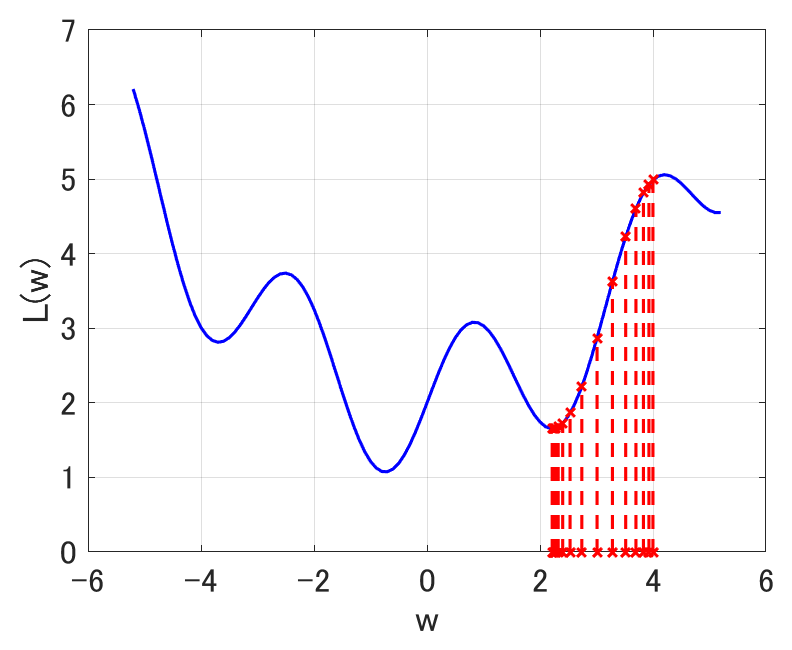
\includegraphics[width=0.8\linewidth]{saikyu12.eps}
  \caption{saikyu12}
  \label{fig:sample7}
\end{figure}

\subsection{考察}

（a）この演習課題をやるにあたり、w、ep、itersの値をそれぞれひとつだけ変化させ、
出力されるグラフにどんな影響があるかを見た。epを変化させたとき、epが大きければ
降下が早く、小さければ降下が遅いことが分かった（図2.1、図2.2）。次にwを変化させると、
ただ初めに調べる場所が変化した（図2.5、図2.6）期値よりも大きすぎる
と、極値を通り過ぎて反対に戻っている様子を伺うことができる。また、反復回数itersを変化
させると探索する回数が変わることが分かる。（図2.3、図2.4）

（b）目的関数を変更したためもちろん描画されるグラフも大きく異なっている。また、三角関数が含まれている
ことで波形がやや複雑になっている。描画したグラフを図2.7に示す。

\section{演習課題1.2}

saikyu21.mのプログラムを以下にしめす。

\begin{lstlisting}[caption=saikyu21.m]
% プログラム1.2: saikyu21.m
%
% 2変数の目的関数対する最急降下法
%
% すべての変数の値を初期化する．グラフをすべて閉じる．
clearvars, close all
% ← (A)
%% 最急降下法
% 初期値，ステップ幅，反復回数の設定
w = [1,1]; % wの初期値
ep = 0.1; % ステップ幅
iters = 20; % 反復回数（number of iterations）
ws = w; % ws: w のすべての値を保存する
% 更新の反復
for i=1:iters
gk = grad(w(1),w(2)); % 勾配の計算
w = w - ep*gk; % 更新
ws = [ws; w]; % 反復点の保存
end

%% 目的関数のグラフを描く
% w: 変数．範囲：-6から0.25刻みで6までのメッシュ範囲
% LW: 目的関数
[w1, w2] = meshgrid(-6:0.25:5.5);
LW = obj_func(w1, w2);
% 目的関数の描画
sc = meshc(w1, w2, LW); hold on
sc(2).LevelList = 2:2:40; % (w1, w2) 平面での等高線の間隔を指定
xlabel('w1'), ylabel('w2'), zlabel('L(W)')
set(gca, 'FontSize', 14)
% ← (B)
%% 結果の描画
for i=1:iters
yk = obj_func(ws(i,1), ws(i,2));
plot3([ws(i,1), ws(i,1)],[ws(i,2),ws(i,2)], [0, yk], 'rx--', 'LineWidth', 1.5)
end
%% (w1, w2) 平面での等高線の描画
figure % 新しい描画ウィンドーを開く
contour(w1, w2, LW, 25), hold on
plot(ws(:,1), ws(:,2), 'rx-', 'LineWidth', 1.5)
xlabel('w1'), ylabel('w2')
set(gca, 'FontSize', 14)
%% 目的関数の計算
function y = obj_func(w1, w2)
y = (w1.^4)/24 + (w2.^4)/32 - w1.^2 - w2.^2 + w1 + w2 + 25; 
end
%
%% 勾配の計算
function g = grad(w1, w2)
g = [(w1.^3)/6 - 2*w1 + 1 , (w2.^3)/8 - 2*w2 + 1]; 
end
%
\end{lstlisting}
（a）初期値wやステップ幅epを様々な値に変更し、最急降下法での収束がどのように変わるかを確かめよ。
必要に応じて、反復回数itersも変更する。

\begin{figure}[H]
  \centering
  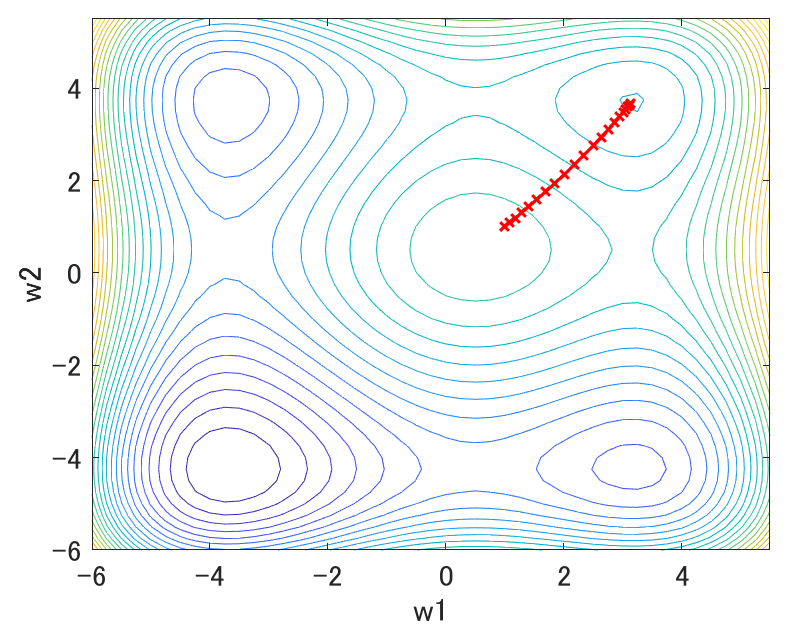
\includegraphics[width=0.8\linewidth]{saikyu21above.eps}
  \caption{saikyu21}
  \label{fig:sample8}
\end{figure}

\begin{figure}[H]
  \centering
  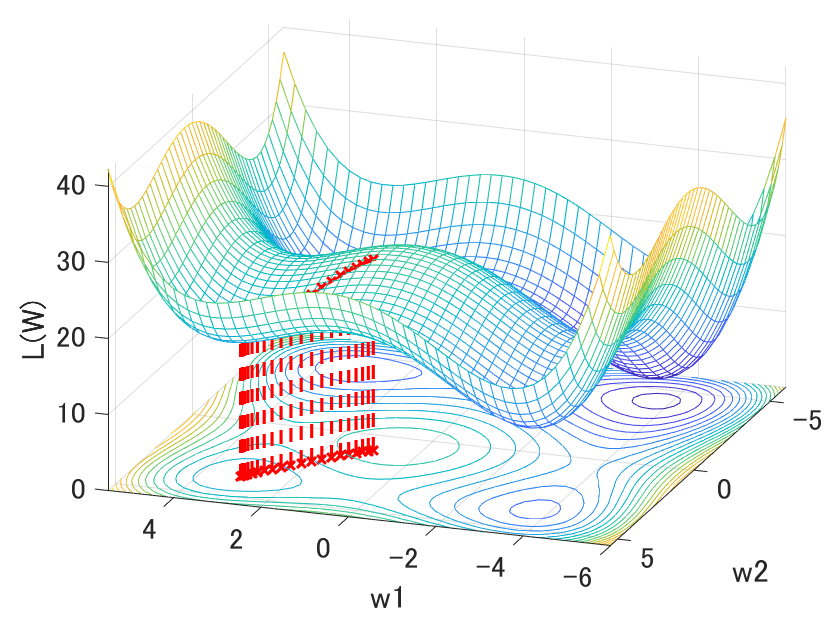
\includegraphics[width=0.8\linewidth]{saikyu21aspect.eps}
  \caption{saikyu21}
  \label{fig:sample9}
\end{figure}

\subsection{考察}

完成したプログラムを実行すると画像（図2.8,2.9）のように出力が得られた。初期値W、ステップ幅ep
を様々な値に変更して最急降下法での収束がどのように変わるかを調べたところ、演習課題1.1で述べた考察
と同じ変化が見られた。

\chapter{第2週：パーセプトロン}

\section{演習課題2.1}

\subsection{（a）}
（a）初期値W,bを変化させて収束の様子を確認する。必要に応じてエポック数を変更する。
また、誤差の範囲を変更し、完全にはクラス分類できない場合があることを確かめよ。\\

\begin{figure}[H]
  \centering
  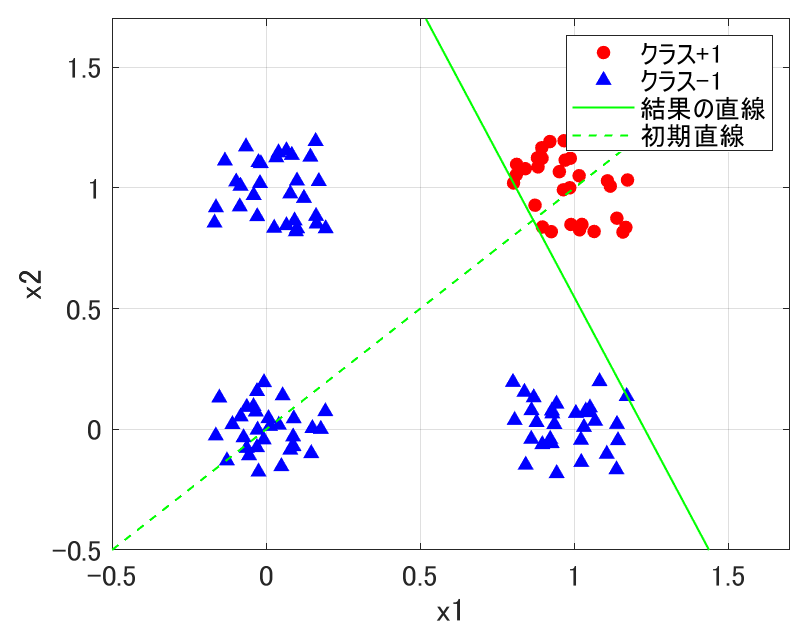
\includegraphics[width=0.8\linewidth]{ptron12.eps}
  \caption{er=0.2}
  \label{fig:sample10}
\end{figure}

\begin{figure}[H]
  \centering
  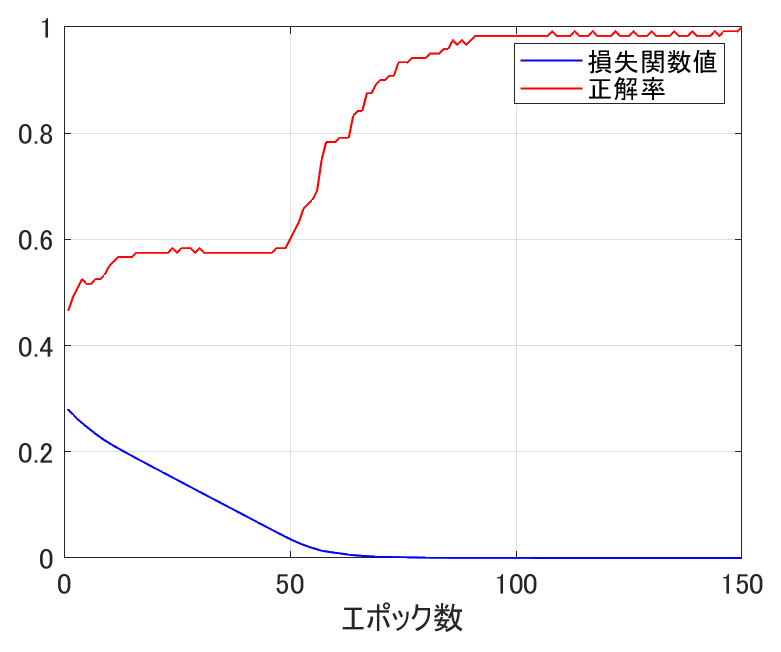
\includegraphics[width=0.8\linewidth]{ptron12g.eps}
  \caption{er=0.2}
  \label{fig:sample11}
\end{figure}

\begin{figure}[H]
  \centering
  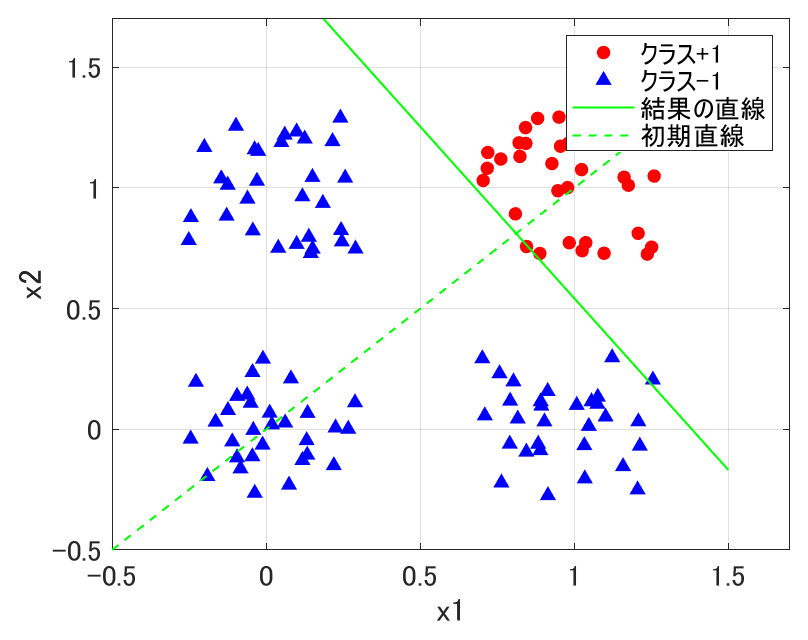
\includegraphics[width=0.8\linewidth]{ptron13.eps}
  \caption{er=0.3}
  \label{fig:sample12}
\end{figure}

\begin{figure}[H]
  \centering
  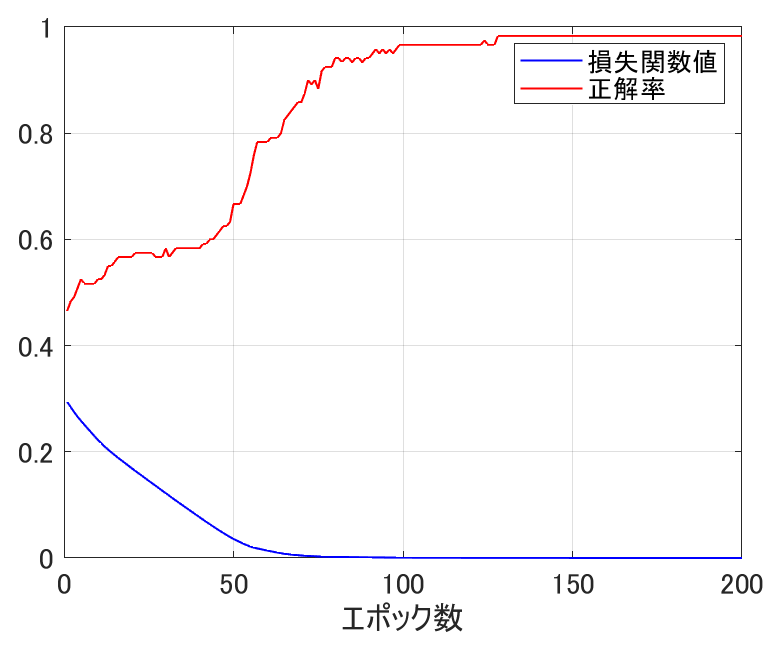
\includegraphics[width=0.8\linewidth]{ptron13g.eps}
  \caption{er=0.3}
  \label{fig:sample13}
\end{figure}

\begin{figure}[H]
  \centering
  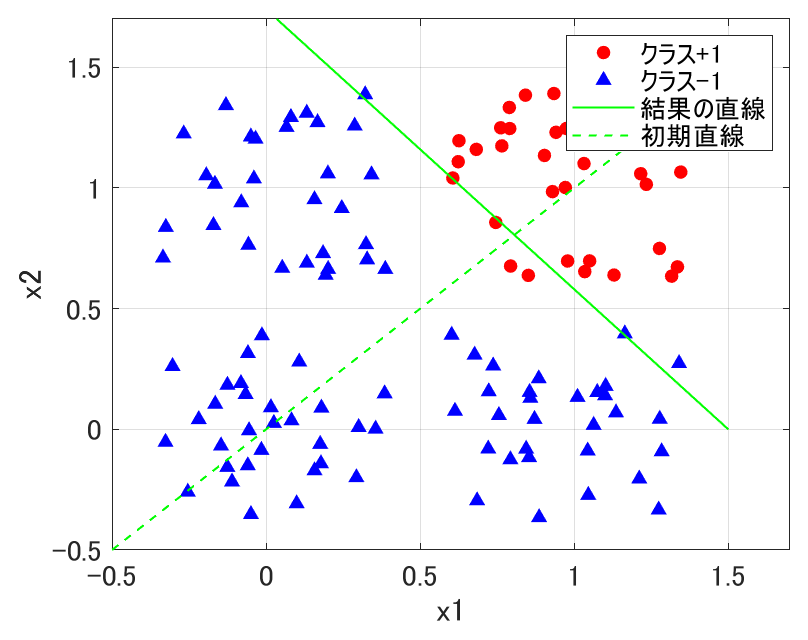
\includegraphics[width=0.8\linewidth]{ptron14.eps}
  \caption{er=0.4}
  \label{fig:sample14}
\end{figure}

\begin{figure}[H]
  \centering
  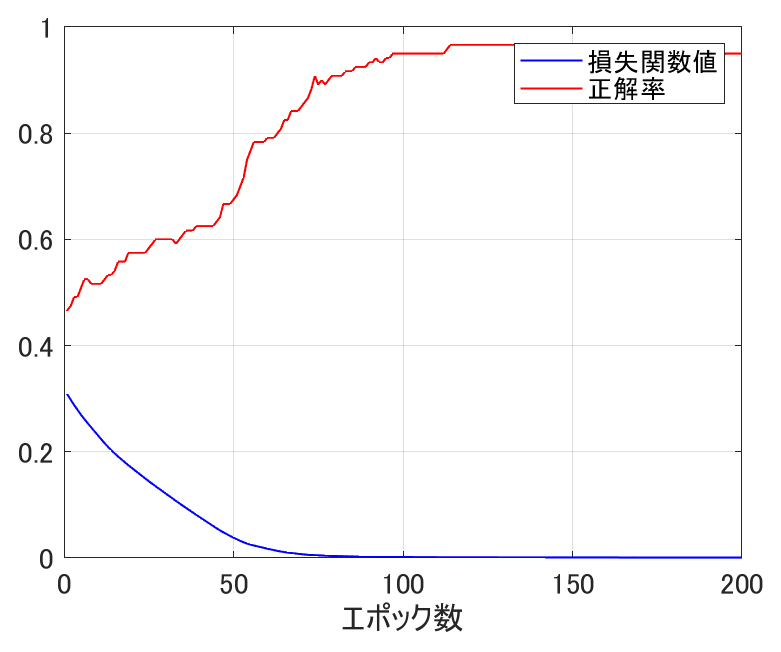
\includegraphics[width=0.8\linewidth]{ptron14g.eps}
  \caption{er=0.4}
  \label{fig:sample15}
\end{figure}

\subsection{考察（a）}

直線の傾きをWが、切片をbが表している。またerは点のばらつきの度合いを表している。
erの値が大きいほどばらつきが大きくなる。私は今回この考察を書くにあたりerが
0.2, 0.3, 0.4のときについて調べた。添付している画像の損失関数を見ると、40から
200ほどまでには0になっていて、期待された値とのずれがないことが見て取れる。このことから
これ以上学習させても正解率があがることが期待されないため、これ以上のクラスタリングは
不可能であると考えられる。

\subsection{（b）}

（b）入力の中ほどにあるtsetをor関係にして、（a）と同様に収束性を確認する。\\

\begin{figure}[H]
  \centering
  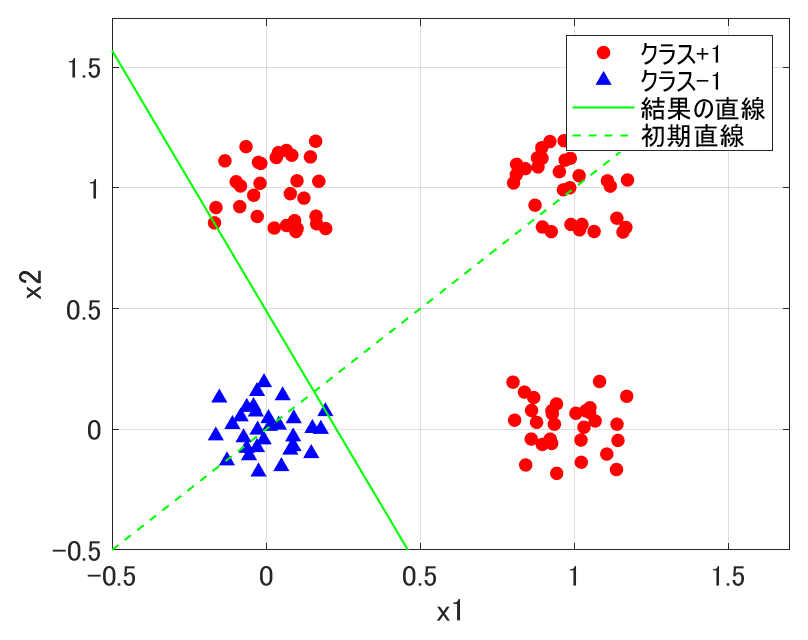
\includegraphics[width=0.8\linewidth]{ptronb.eps}
  \caption{or関係}
  \label{fig:sample16}
\end{figure}

\begin{figure}[H]
  \centering
  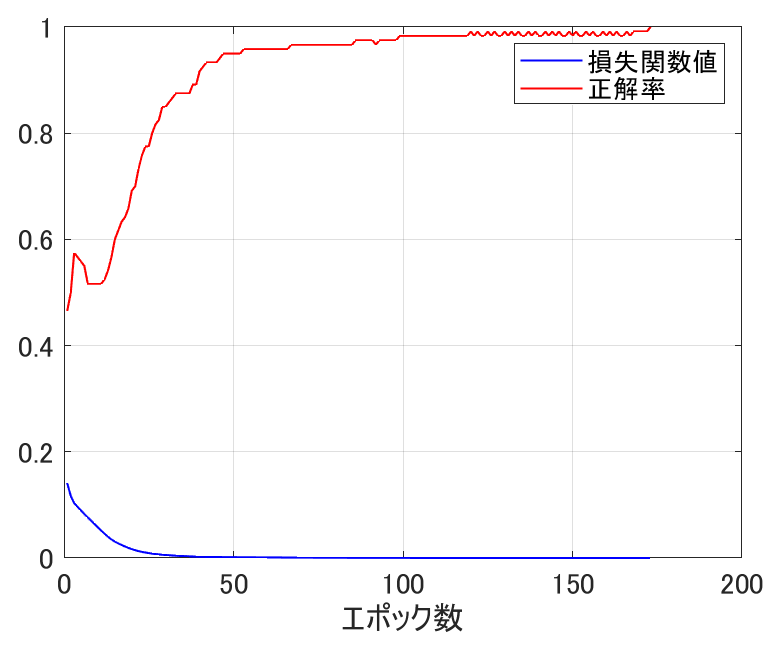
\includegraphics[width=0.8\linewidth]{ptronbg.eps}
  \caption{or関係}
  \label{fig:sample17}
\end{figure}

\subsection{考察（b）}

and関係からor関係に変更して、プログラムを実行した。実行して得られた損失関数と正解率のグラフ
を見ると、収束の仕方はand関係のグラフと変らないように見える。

\subsection{（c）}

（c）上記プログラムをオンライン学習やミニバッチ学習に変更せよ。ミニバッチ学習の場合、
例えばバッチサイズを20や30として実行せよ。\\

\begin{figure}[H]
  \centering
  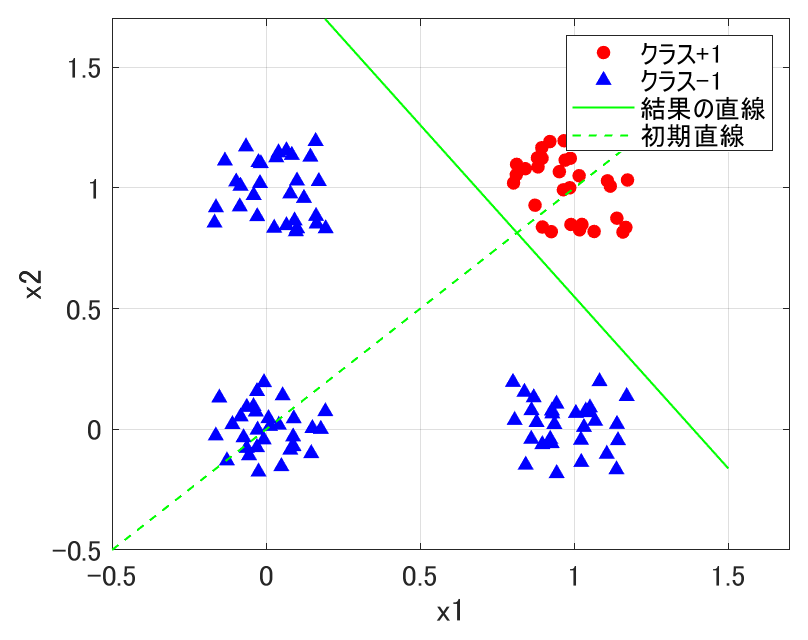
\includegraphics[width=0.8\linewidth]{online.eps}
  \caption{オンライン学習}
  \label{fig:sample18}
\end{figure}

\begin{figure}[H]
  \centering
  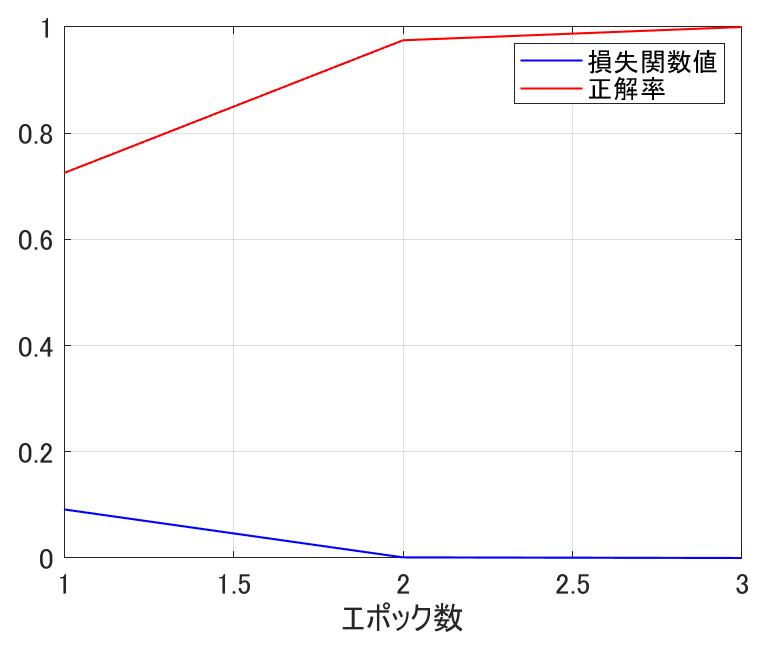
\includegraphics[width=0.8\linewidth]{onlineg.eps}
  \caption{オンライン学習}
  \label{fig:sample19}
\end{figure}

\begin{figure}[H]
  \centering
  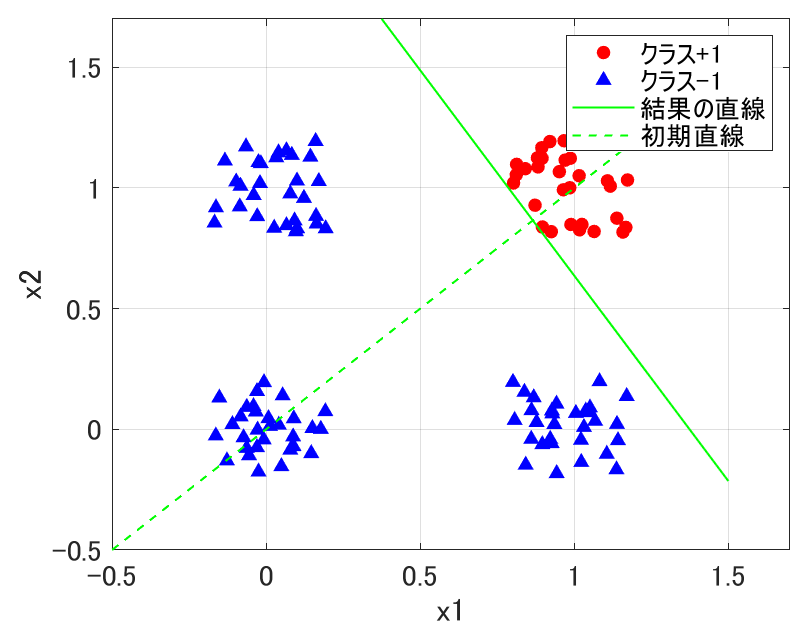
\includegraphics[width=0.8\linewidth]{mini.eps}
  \caption{ミニバッチ学習}
  \label{fig:sample20}
\end{figure}

\begin{figure}[H]
  \centering
  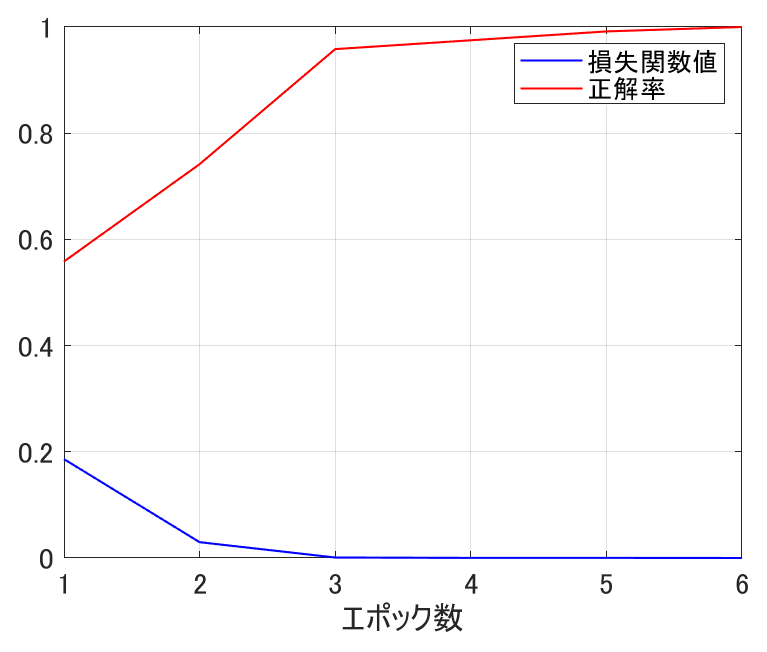
\includegraphics[width=0.8\linewidth]{minig.eps}
  \caption{ミニバッチ学習}
  \label{fig:sample21}
\end{figure}

\subsection{考察（c）}

オンライン学習とミニバッチ学習はどちらもバッチ学習よりもエポック数が少なくなる学習方法ですが、
ある一定の区間をまとめてバッチ学習をして、その処理を繰り返しているミニバッチ学習のほうが、オンライン学習
寄りもエポック数が多くなっている。それぞれのアルゴリズムをみればこの結果が出た理由が良くわかると
思った。特にバッチ学習は全データを見ることでエポック数が一番多くなる、という結果が顕著にグラフに
表れているように見える。

\chapter{第3週：多層ニューラルネットワーク}

\section{演習課題3.1（a）}

\begin{figure}[H]
  \centering
  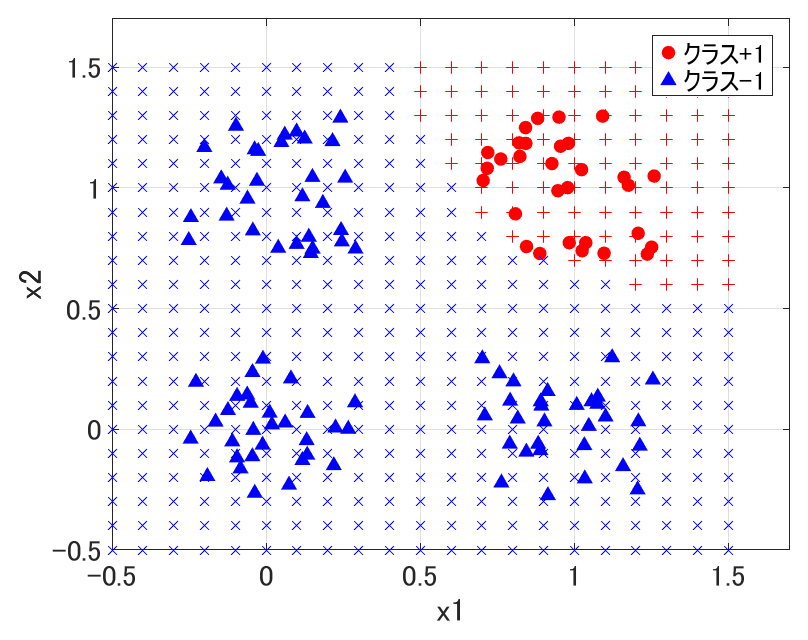
\includegraphics[width=0.8\linewidth]{N33.eps}
  \caption{3層NN,dimlayer=50,numEpochs=200,er=0.3}
  \label{fig:sample22}
\end{figure}

\begin{figure}[H]
  \centering
  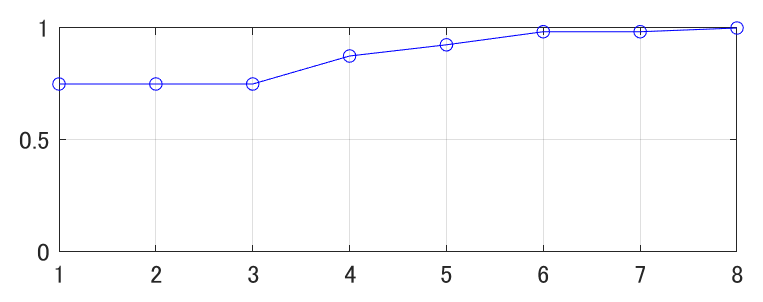
\includegraphics[width=0.8\linewidth]{N33ga.eps}
  \caption{3層NN,dimlayer=50,numEpochs=200,er=0.3}
  \label{fig:sample23}
\end{figure}

\begin{figure}[H]
  \centering
  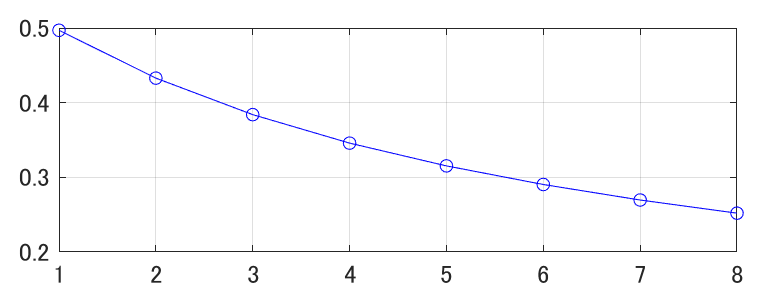
\includegraphics[width=0.8\linewidth]{N33gb.eps}
  \caption{3層NN,dimlayer=50,numEpochs=200,er=0.3}
  \label{fig:sample24}
\end{figure}

\begin{figure}[H]
  \centering
  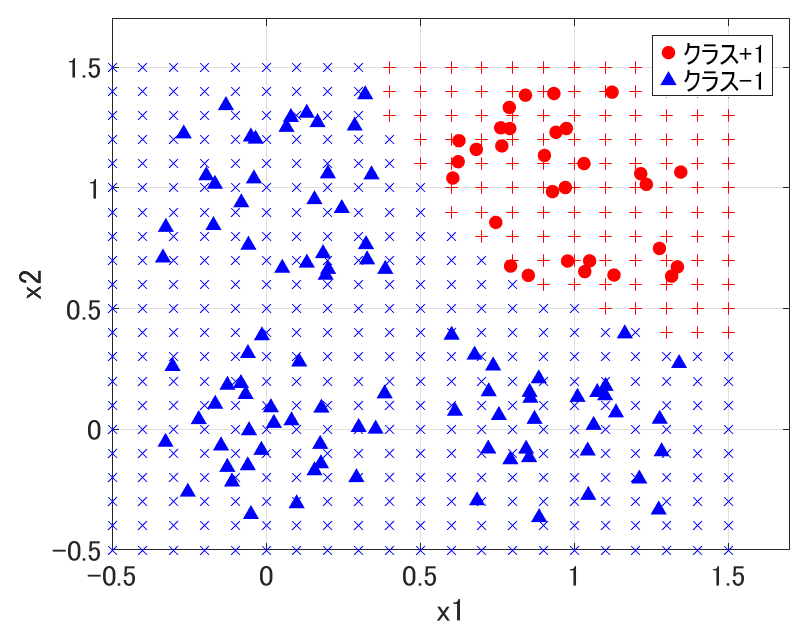
\includegraphics[width=0.8\linewidth]{N34.eps}
  \caption{3層NN,dimlayer=50,numEpochs=200,er=0.4}
  \label{fig:sample25}
\end{figure}

\begin{figure}[H]
  \centering
  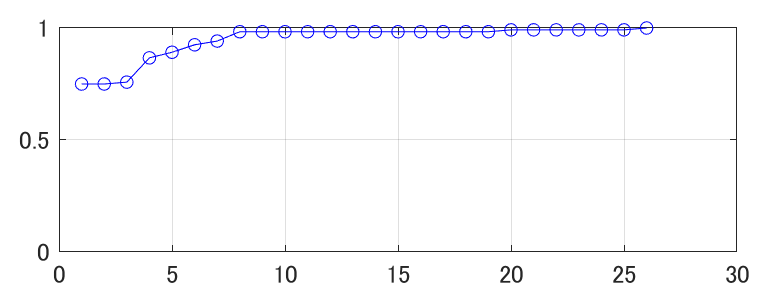
\includegraphics[width=0.8\linewidth]{N34ga.eps}
  \caption{3層NN,dimlayer=50,numEpochs=200,er=0.4}
  \label{fig:sample26}
\end{figure}

\begin{figure}[H]
  \centering
  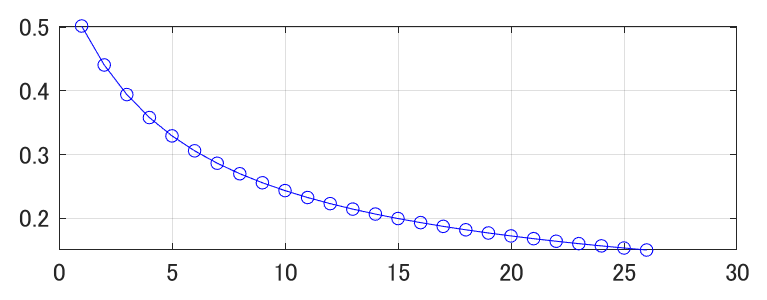
\includegraphics[width=0.8\linewidth]{N34gb.eps}
  \caption{3層NN,dimlayer=50,numEpochs=200,er=0.4}
  \label{fig:sample27}
\end{figure}

\begin{figure}[H]
  \centering
  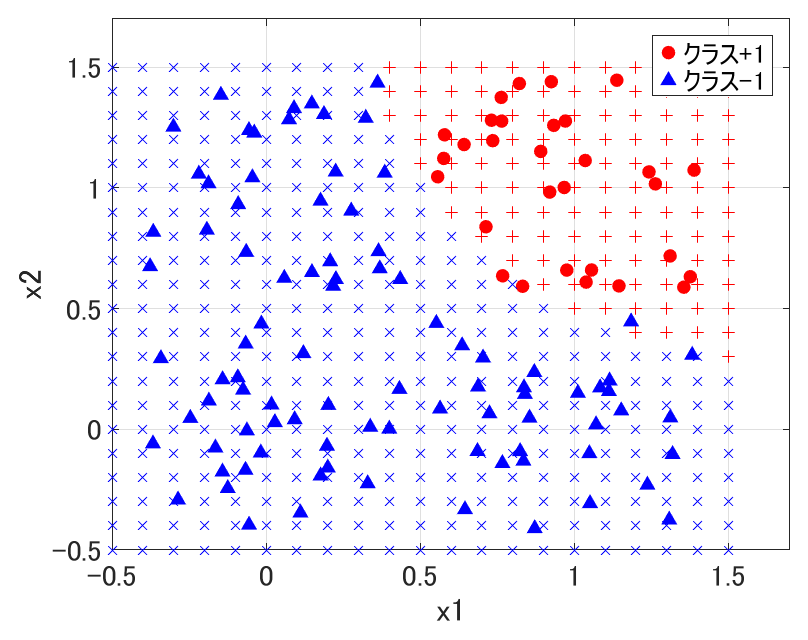
\includegraphics[width=0.8\linewidth]{N345.eps}
  \caption{3層NN,dimlayer=50,numEpochs=200,er=0.45}
  \label{fig:sample28}
\end{figure}

\begin{figure}[H]
  \centering
  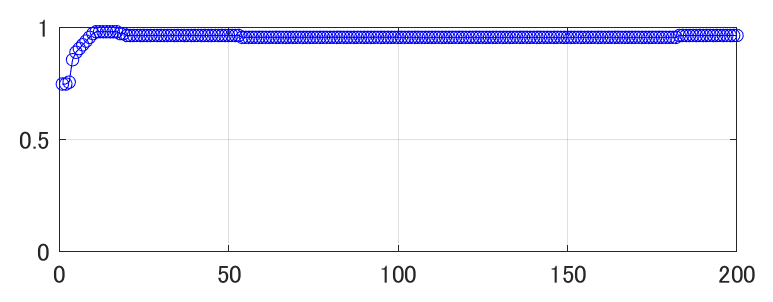
\includegraphics[width=0.8\linewidth]{N345ga.eps}
  \caption{3層NN,dimlayer=50,numEpochs=200,er=0.45}
  \label{fig:sample29}
\end{figure}

\begin{figure}[H]
  \centering
  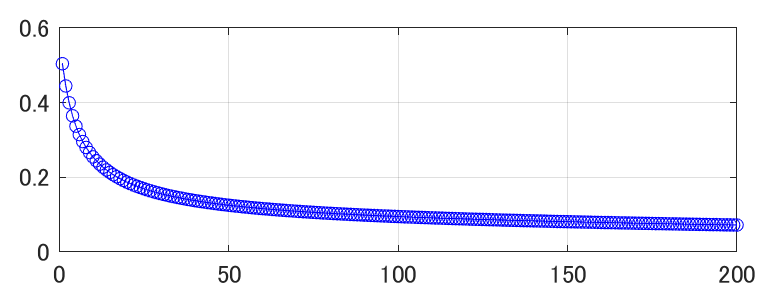
\includegraphics[width=0.8\linewidth]{N345gb.eps}
  \caption{3層NN,dimlayer=50,numEpochs=200,er=0.45}
  \label{fig:sample30}
\end{figure}

\begin{figure}[H]
  \centering
  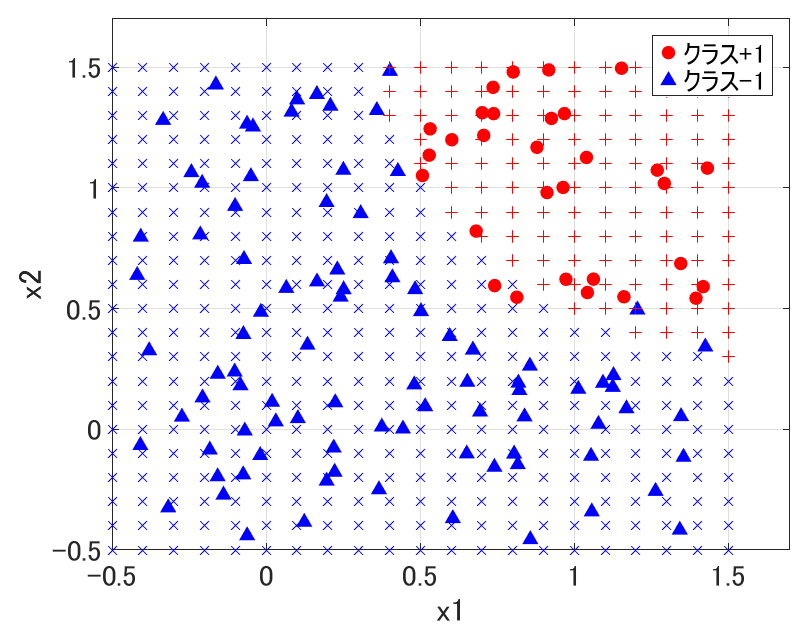
\includegraphics[width=0.8\linewidth]{N35.eps}
  \caption{3層NN,dimlayer=50,numEpochs=200,er=0.5}
  \label{fig:sample31}
\end{figure}

\begin{figure}[H]
  \centering
  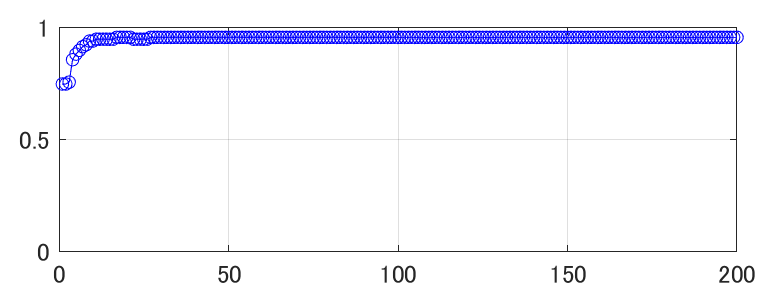
\includegraphics[width=0.8\linewidth]{N35ga.eps}
  \caption{3層NN,dimlayer=50,numEpochs=200,er=0.5}
  \label{fig:sample32}
\end{figure}

\begin{figure}[H]
  \centering
  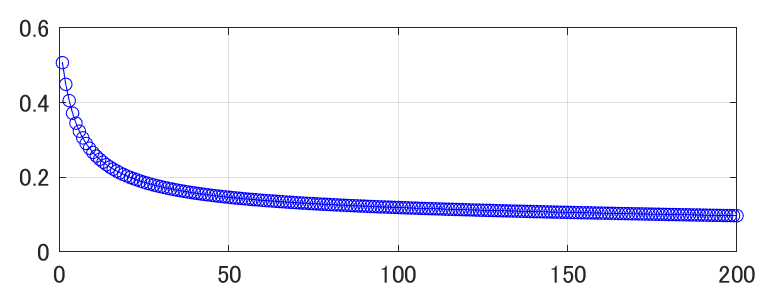
\includegraphics[width=0.8\linewidth]{N35gb.eps}
  \caption{3層NN,dimlayer=50,numEpochs=200,er=0.5}
  \label{fig:sample33}
\end{figure}

\begin{figure}[H]
  \centering
  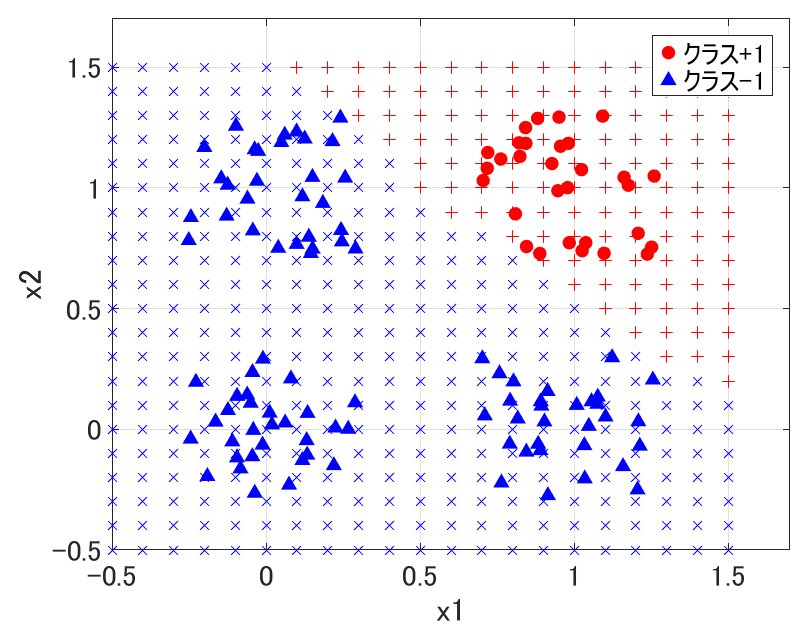
\includegraphics[width=0.8\linewidth]{N33100.eps}
  \caption{3層NN,dimlayer=100,numEpochs=200,er=0.3}
  \label{fig:sample34}
\end{figure}

\begin{figure}[H]
  \centering
  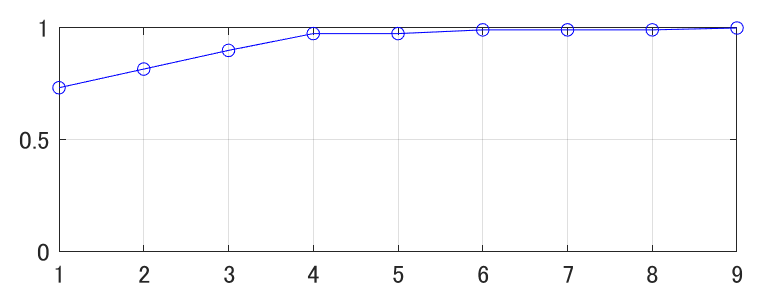
\includegraphics[width=0.8\linewidth]{N33100ga.eps}
  \caption{3層NN,dimlayer=100,numEpochs=200,er=0.3}
  \label{fig:sample35}
\end{figure}

\begin{figure}[H]
  \centering
  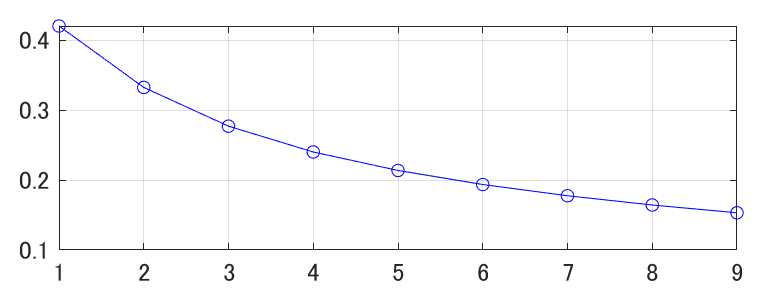
\includegraphics[width=0.8\linewidth]{N33100gb.eps}
  \caption{3層NN,dimlayer=100,numEpochs=200,er=0.3}
  \label{fig:sample36}
\end{figure}

\begin{figure}[H]
  \centering
  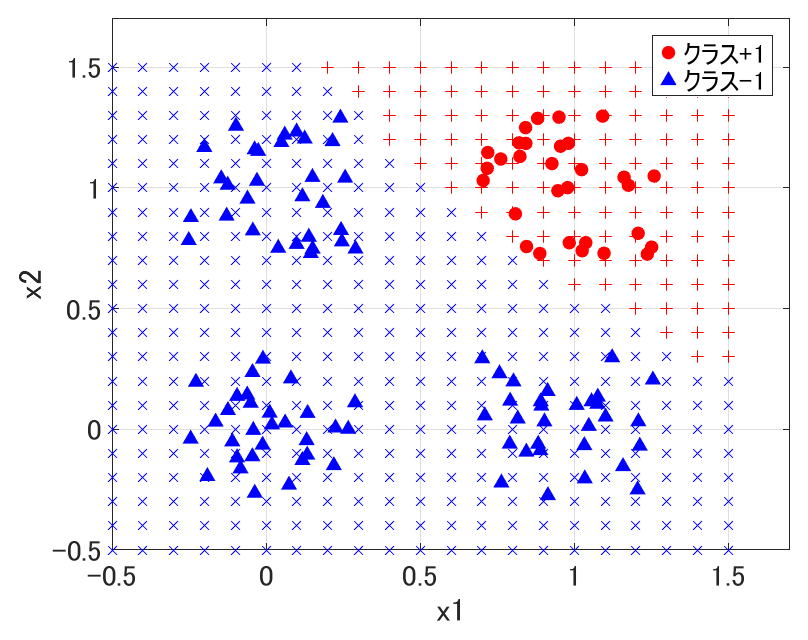
\includegraphics[width=0.8\linewidth]{N3200.eps}
  \caption{3層NN,dimlayer=200,numEpochs=200,er=0.3}
  \label{fig:sample37}
\end{figure}

\begin{figure}[H]
  \centering
  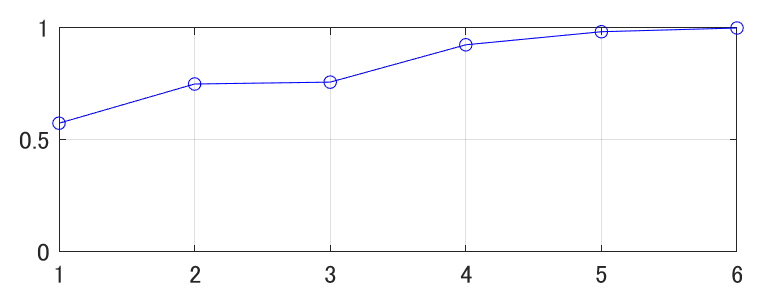
\includegraphics[width=0.8\linewidth]{N3200ga.eps}
  \caption{3層NN,dimlayer=200,numEpochs=200,er=0.3}
  \label{fig:sample38}
\end{figure}

\begin{figure}[H]
  \centering
  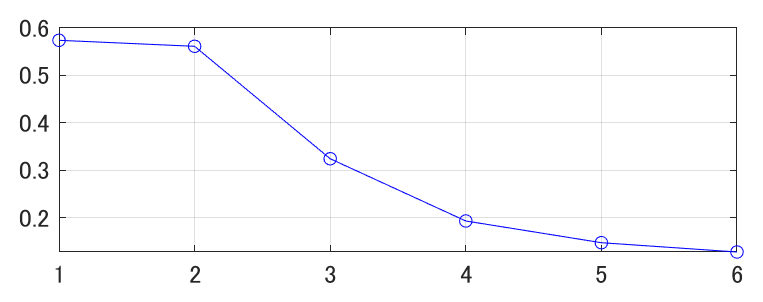
\includegraphics[width=0.8\linewidth]{N3200gb.eps}
  \caption{3層NN,dimlayer=200,numEpochs=200,er=0.3}
  \label{fig:sample39}
\end{figure}

\begin{figure}[H]
  \centering
  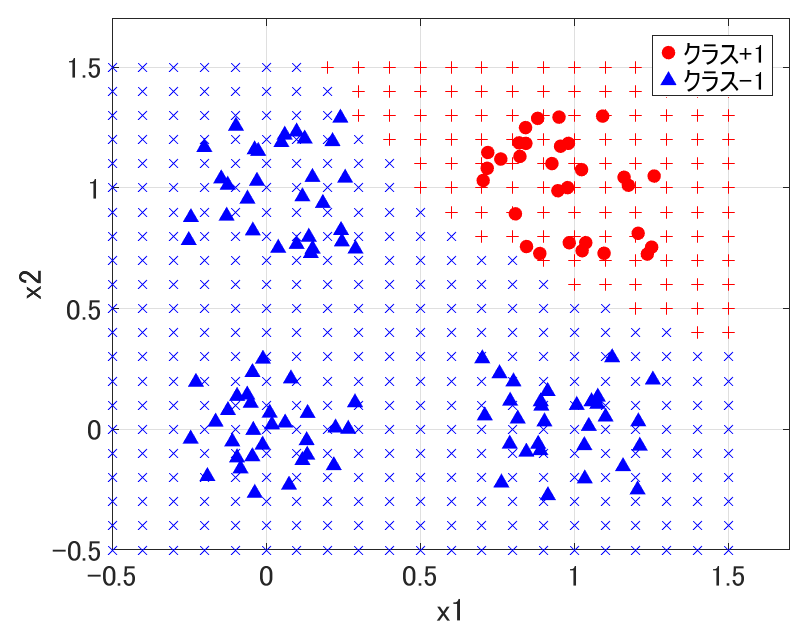
\includegraphics[width=0.8\linewidth]{N3500.eps}
  \caption{3層NN,dimlayer=500,numEpochs=200,er=0.3}
  \label{fig:sample40}
\end{figure}

\begin{figure}[H]
  \centering
  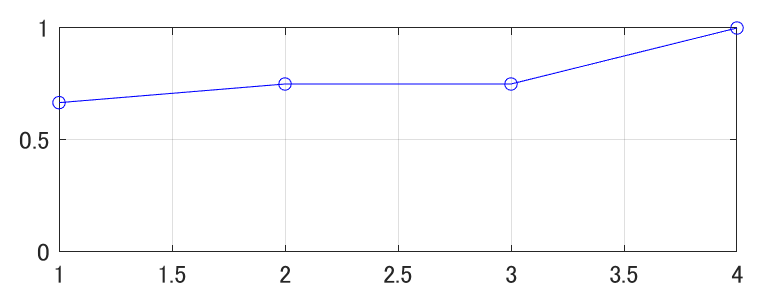
\includegraphics[width=0.8\linewidth]{N3500ga.eps}
  \caption{3層NN,dimlayer=500,numEpochs=200,er=0.3}
  \label{fig:sample41}
\end{figure}

\begin{figure}[H]
  \centering
  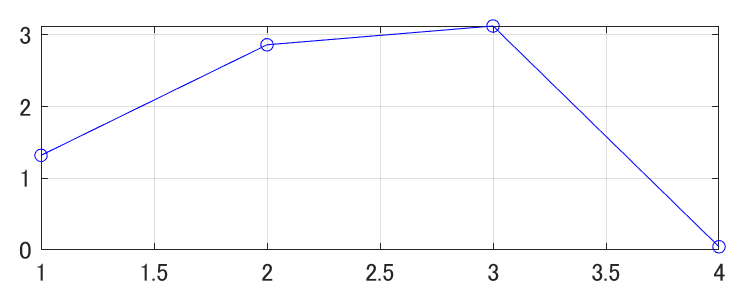
\includegraphics[width=0.8\linewidth]{N3500gb.eps}
  \caption{3層NN,dimlayer=500,numEpochs=200,er=0.3}
  \label{fig:sample42}
\end{figure}

\begin{figure}[H]
  \centering
  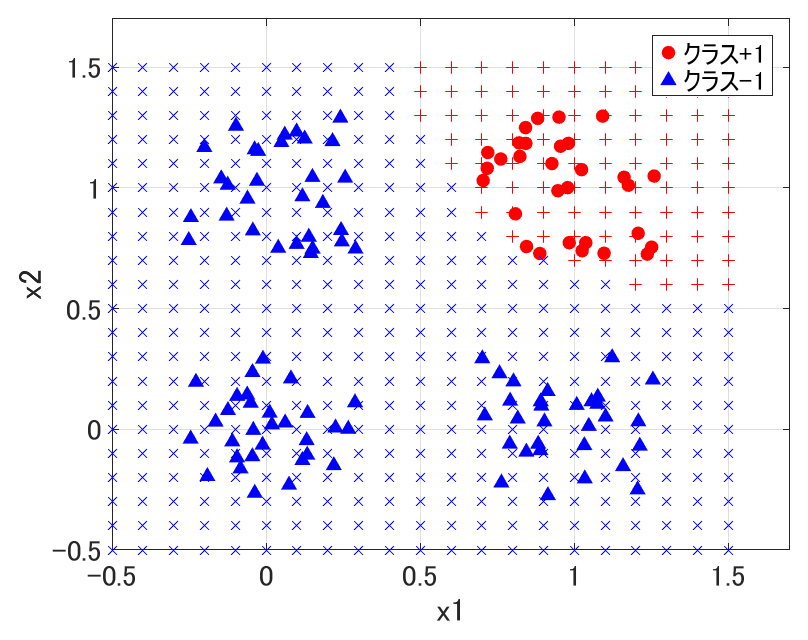
\includegraphics[width=0.8\linewidth]{N3epo100.eps}
  \caption{3層NN,dimlayer=500,numEpochs=100,er=0.3}
  \label{fig:sample43}
\end{figure}

\begin{figure}[H]
  \centering
  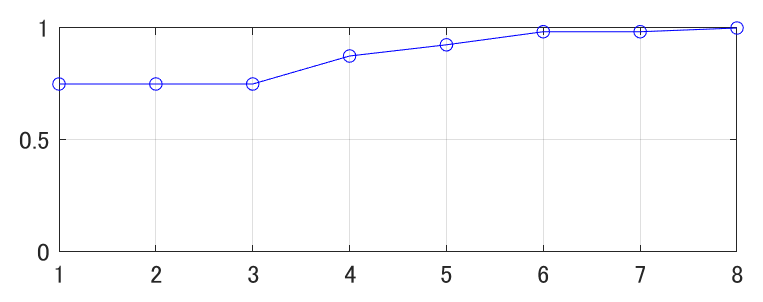
\includegraphics[width=0.8\linewidth]{N3epo100ga.eps}
  \caption{3層NN,dimlayer=500,numEpochs=100,er=0.3}
  \label{fig:sample44}
\end{figure}

\begin{figure}[H]
  \centering
  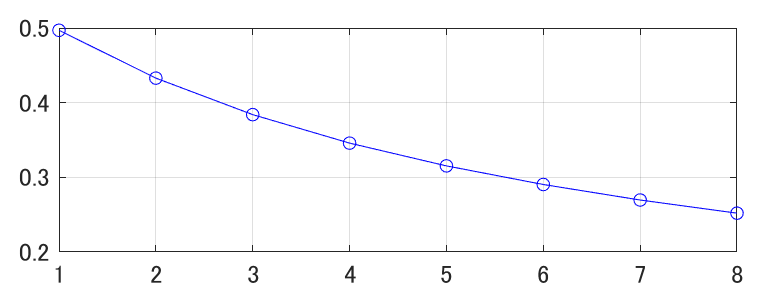
\includegraphics[width=0.8\linewidth]{N3epo100gb.eps}
  \caption{3層NN,dimlayer=500,numEpochs=100,er=0.3}
  \label{fig:sample45}
\end{figure}

\section{考察（a）}

誤差erとnumEpochsが同じであるときに、中間ノードが大きくなれば正解率が 1 になるまで
のエポック数が小さくなることはすべてに当てはまった。中間ノードの値が大きくなれば分類
精度が高くなっていることがわかった。
しかし中間ノードの値が大きくなったとしても分類精度は変わっていない。
これは前者が偶発的だった可能性がある。中間ノードの変化は分類精度と正解率が 1 になるま
でのエポック数両方に変化をもたらす。具体的には中間ノードが大きくなれば分類
精度が高く、エポック数が小さく、中間ノードが小さくなればその逆が起こることがわかった。

\section{演習課題3.1（b）}

作成した3層ニューラルネットワークのプログラムを4層ニューラルネットワーク（2層の中間層）
に拡張せよ。そして、中間層1、2のノード数を50、100、200、500などの組み合わせで変化させ、
分類精度の違いについて確認せよ。また、中間層1層では完全に分類できなかった場合でも、
中間層を2層にすることにより完全に分類できるようになる場合があることも確認せよ。




\chapter{第4週：手書き文字数字認識への拡張}

　Matlabの手書き数字ベースを用い、「0、1、2、3、4、5、6、7、8、9」の10個の数字に
分類する10クラス分類プログラムを作成する。

\section{演習課題4.1}
（a）上記のプログラムを作成し、中間層のノード数やエポック数を変化させ、テストデータの分類
精度が高くなるように工夫せよ。なお、今回の学習は各エポックの計算に時間がかかるので時間の使い方
に注意せよ

\section{演習課題4.2}
（a）tryPredictを実行し、様々な数字を入力し、その推定能力を確認する。



\end{document}
